\part{Fundamental Principles}

\chapter{Human Vision and Perception}

\section{Introduction}

The human visual system represents the ultimate specification for display technology. Understanding its capabilities and limitations is essential for optimal display engineering. This chapter provides comprehensive coverage of visual psychophysics and its implications for display design.

\begin{definitionbox}{Trichromatic Vision}
Human color vision is based on three cone types with overlapping spectral sensitivities:
\begin{itemize}[leftmargin=*]
  \item \textbf{S-cones} (short wavelength): Peak sensitivity at $\lambda_S \approx 420$ nm
  \item \textbf{M-cones} (medium wavelength): Peak sensitivity at $\lambda_M \approx 534$ nm
  \item \textbf{L-cones} (long wavelength): Peak sensitivity at $\lambda_L \approx 564$ nm
\end{itemize}
The combination of signals from these three receptor types enables perception of approximately $10^7$ distinct colors.
\end{definitionbox}

\subsection{Photoreceptor Characteristics}

The human retina contains approximately 120 million rods and 6 million cones, distributed non-uniformly across the retinal surface.

\begin{figure}[H]
\centering
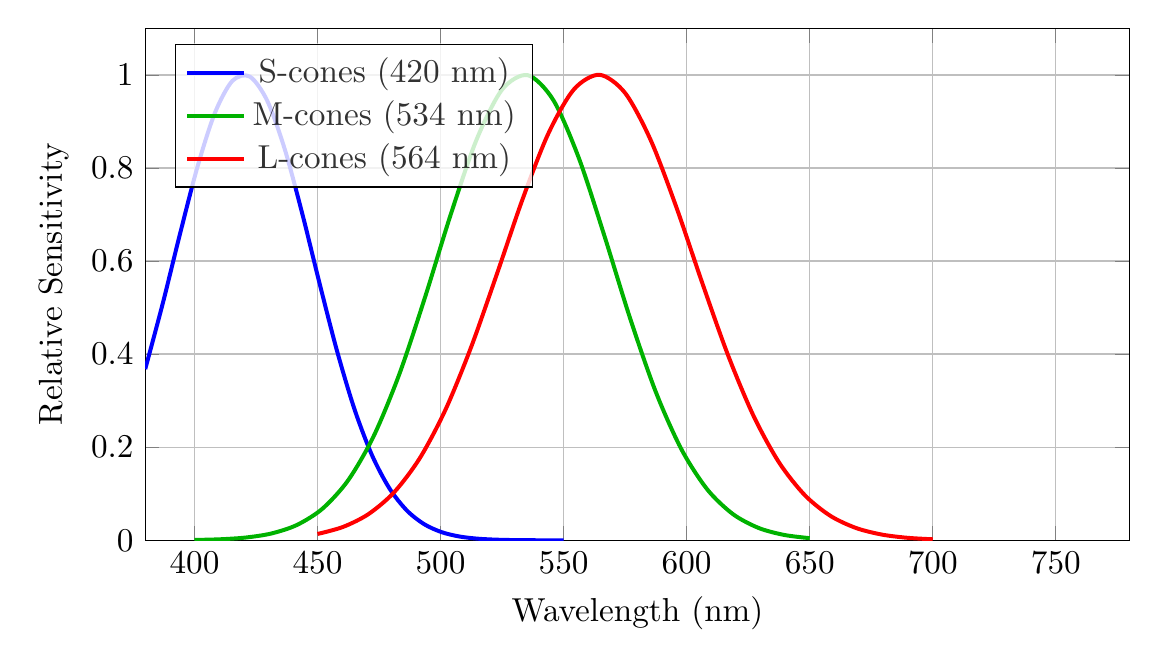
\begin{tikzpicture}[scale=1.2]
  \begin{axis}[
    width=12cm,
    height=7cm,
    xlabel={Wavelength (nm)},
    ylabel={Relative Sensitivity},
    xmin=380, xmax=780,
    ymin=0, ymax=1.1,
    grid=major,
    legend pos=north west,
    legend style={fill=white, fill opacity=0.8}
  ]
  
  % S-cone
  \addplot[color=blue, very thick, smooth, domain=380:550] 
    {exp(-((x-420)/40)^2)};
  \addlegendentry{S-cones (420 nm)}
  
  % M-cone
  \addplot[color=green!70!black, very thick, smooth, domain=400:650] 
    {exp(-((x-534)/50)^2)};
  \addlegendentry{M-cones (534 nm)}
  
  % L-cone
  \addplot[color=red, very thick, smooth, domain=450:700] 
    {exp(-((x-564)/55)^2)};
  \addlegendentry{L-cones (564 nm)}
  
  \end{axis}
\end{tikzpicture}
\caption{Spectral sensitivity curves for the three cone types in human vision. Note the significant overlap between M and L cones, which enables fine color discrimination in the yellow-green region.}
\label{fig:cone_sensitivity}
\end{figure}

\subsection{Spatial Resolution}

Peak foveal acuity achieves approximately 1 arcminute resolution, corresponding to:

\begin{formulabox}{Required Display PPI}
For a display at viewing distance $d$ (inches), the required pixel density to achieve ``Retina'' quality (imperceptible pixels) is:
\begin{equation}
  \text{PPI}_{\text{required}} = \frac{60 \text{ pixels/degree} \times 180}{\pi \times d} = \frac{3438}{d}
\end{equation}

\textbf{Examples:}
\begin{itemize}
  \item Smartphone at 12 inches: $\text{PPI} = 3438/12 = 286$
  \item Laptop at 24 inches: $\text{PPI} = 3438/24 = 143$
  \item Desktop monitor at 30 inches: $\text{PPI} = 3438/30 = 115$
  \item VR headset at 2 inches: $\text{PPI} = 3438/2 = 1719$
\end{itemize}
\end{formulabox}

\begin{figure}[H]
\centering
\begin{tikzpicture}
  \begin{axis}[
    width=12cm,
    height=8cm,
    xlabel={Viewing Distance (inches)},
    ylabel={Required PPI},
    xmin=0, xmax=40,
    ymin=0, ymax=400,
    grid=major,
    legend pos=north east
  ]
  
  \addplot[color=primarycolor, very thick, domain=6:40] {3438/x};
  \addlegendentry{Retina threshold}
  
  % Mark common devices
  \addplot[only marks, mark=*, mark size=3pt, color=accentcolor] 
    coordinates {(12,286) (24,143) (30,115)};
  
  \node[above right] at (axis cs:12,286) {\small Phone};
  \node[above right] at (axis cs:24,143) {\small Laptop};
  \node[above right] at (axis cs:30,115) {\small Monitor};
  
  \end{axis}
\end{tikzpicture}
\caption{Required pixel density versus viewing distance to achieve imperceptible pixels. Real devices typically exceed this threshold for marketing purposes.}
\label{fig:ppi_requirement}
\end{figure}

\subsection{Contrast Sensitivity Function}

The human visual system exhibits a band-pass contrast sensitivity function (CSF), with peak sensitivity around 4 cycles per degree.

\begin{examplebox}{Practical Implication}
This band-pass characteristic means that:
\begin{enumerate}
  \item Very low spatial frequencies (large features) are less perceptible than mid-frequencies
  \item Very high spatial frequencies (fine details) fall off rapidly
  \item Anti-aliasing is most critical for frequencies near the CSF peak
  \item Subpixel rendering effectively triples horizontal resolution exactly where it matters most
\end{enumerate}
\end{examplebox}

\section{Psychophysical Laws}

\subsection{Weber-Fechner Law}

The relationship between physical stimulus and perceived sensation:

\begin{formulabox}{Weber-Fechner Law}
\begin{equation}
  S = k \ln\left(\frac{I}{I_0}\right)
\end{equation}
where:
\begin{itemize}
  \item $S$ = perceived sensation magnitude
  \item $I$ = physical stimulus intensity
  \item $I_0$ = threshold intensity
  \item $k$ = Weber constant
\end{itemize}

\textbf{Weber Fraction for Brightness:} $\Delta L / L \approx 0.01$ to $0.02$ (1--2\%)
\end{formulabox}

\subsection{Stevens' Power Law}

A more accurate model, especially at higher intensities:

\begin{formulabox}{Stevens' Power Law}
\begin{equation}
  \psi = k \phi^n
\end{equation}
where:
\begin{itemize}
  \item $\psi$ = perceived magnitude
  \item $\phi$ = physical magnitude
  \item $n$ = modality-specific exponent
  \item $k$ = proportionality constant
\end{itemize}

\textbf{For brightness perception:} $n \approx 0.33$
\end{formulabox}

\begin{importantbox}{Connection to Gamma Correction}
Stevens' power law with $n = 0.33$ for brightness implies that for perceptually uniform encoding:
\begin{equation}
  V \propto \psi \propto L^{0.33} \quad \Rightarrow \quad L \propto V^{1/0.33} \approx V^{3.0}
\end{equation}

The standard display gamma of $\gamma = 2.2$ represents a compromise between:
\begin{itemize}
  \item Perceptual uniformity ($\gamma \approx 3.0$)
  \item CRT physics ($\gamma \approx 2.5$)
  \item Practical considerations (bit depth, surround conditions)
\end{itemize}
\end{importantbox}

% ============================================================================
% CHAPTER 2: RADIOMETRY AND PHOTOMETRY
% ============================================================================
